\documentclass{article}
\usepackage{tikz}
\usetikzlibrary{positioning}
\tikzstyle{block} = [draw, minimum width = 2cm, minimum height = 1.2cm, fill=blue!5]
\tikzstyle{sum} = [draw, fill=blue!5, circle, node distance=1cm]
\begin{document}
\begin{figure}[h]\centering
    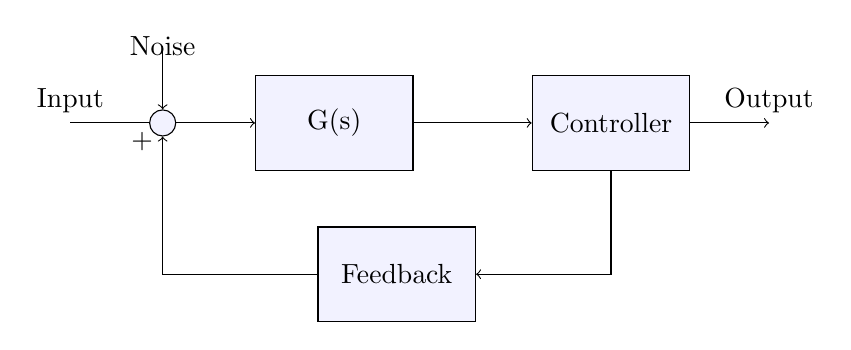
\begin{tikzpicture}
        %Blocks
        \node [block] (G) at (0,0) {G(s)};
        \node [block, right = 1.5 cm of G,] (controller) {Controller};
        \node [block, below left = 1 cm of controller] (feedback) {Feedback} ;
        \node [sum, left = of G] (sum) {};
        %Arrows
        \draw[->] (G) -- (controller);
        \draw[->] (controller.east) -- ++(1.0,0) node [right,above](){Output};
        \draw[->] (controller.south) |- (feedback.east) ;
        \draw[->] (feedback.west) -| (sum) node[below left](){+};
        \draw[->] (sum.west) ++ (-1,0) node[above](){Input}-- (sum.west)
            (sum.east) -- (G.west)
        ;
        \draw[->] (sum.north) ++ (0,0.8) node{Noise} -- (sum.north);
    \end{tikzpicture}
\end{figure}
\end{document}